\documentclass[tikz,border=3pt]{standalone}
\usepackage[utf8]{inputenc}
\usepackage[T1]{fontenc}
\usepackage{lmodern}
\renewcommand{\familydefault}{\sfdefault}
\usepackage{sansmath}\sansmath
\usepackage{chemfig}
\usepackage{pgfplots}\pgfplotsset{compat=1.18,/pgf/number format/use comma,/pgf/number format/1000 sep={.}}
\usetikzlibrary{arrows.meta,calc,positioning,decorations.pathmorphing,patterns}
% paleta del sitio
\definecolor{nar}{HTML}{E8680C}\definecolor{narc}{HTML}{FFB35C}\definecolor{hielo}{HTML}{FFF3E8}
\definecolor{tinta}{HTML}{1D1D1F}\definecolor{gris}{HTML}{6E6E73}\definecolor{lila}{HTML}{7C5CF0}
\definecolor{azul}{HTML}{2F6FD6}\definecolor{menta}{HTML}{17A673}\definecolor{coral}{HTML}{E8342A}
\tikzset{cel/.style={draw=gris,fill=hielo,line width=0.9pt},nuc/.style={draw=gris!70,line width=0.6pt},
fib/.style={gris!55,line width=0.35pt},eti/.style={font=\footnotesize,text=tinta,align=center},
num/.style={circle,draw=nar,fill=white,text=nar,font=\small\bfseries,inner sep=1.2pt,minimum size=13pt},
fl/.style={-{Stealth[length=2.6mm]},gris,line width=0.9pt}}
\begin{document}
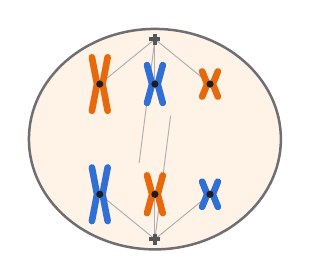
\begin{tikzpicture}[font=\small]
\draw[cel] (0,0) ellipse (1.6 and 1.4);
\draw[fib] (0,1.27)--(-0.7,0.7);
\draw[fib] (0,-1.27)--(-0.7,-0.7);
\draw[fib] (0,1.27)--(0,0.7);
\draw[fib] (0,-1.27)--(0,-0.7);
\draw[fib] (0,1.27)--(0.7,0.7);
\draw[fib] (0,-1.27)--(0.7,-0.7);
\draw[fib] (0,1.27)--(-0.2,-0.3);
\draw[fib] (0,-1.27)--(0.2,0.3);
\begin{scope}[shift={(-0.7,0.7)},rotate=0]\draw[nar,line width=2.4pt,line cap=round,line join=round] (-0.1,0.34)--(-0.035,0)--(-0.1,-0.34);\end{scope}
\begin{scope}[shift={(-0.7,0.7)},rotate=0]\draw[nar,line width=2.4pt,line cap=round,line join=round] (0.1,0.34)--(0.035,0)--(0.1,-0.34);\end{scope}
\fill[tinta] (-0.7,0.7) circle (1.3pt);
\begin{scope}[shift={(-0.7,-0.7)},rotate=0]\draw[azul,line width=2.4pt,line cap=round,line join=round] (-0.1,0.34)--(-0.035,0)--(-0.1,-0.34);\end{scope}
\begin{scope}[shift={(-0.7,-0.7)},rotate=0]\draw[azul,line width=2.4pt,line cap=round,line join=round] (0.1,0.34)--(0.035,0)--(0.1,-0.34);\end{scope}
\fill[tinta] (-0.7,-0.7) circle (1.3pt);
\begin{scope}[shift={(0,0.7)},rotate=0]\draw[azul,line width=2.4pt,line cap=round,line join=round] (-0.1,0.24)--(-0.035,0)--(-0.1,-0.24);\end{scope}
\begin{scope}[shift={(0,0.7)},rotate=0]\draw[azul,line width=2.4pt,line cap=round,line join=round] (0.1,0.24)--(0.035,0)--(0.1,-0.24);\end{scope}
\fill[tinta] (0,0.7) circle (1.3pt);
\begin{scope}[shift={(0,-0.7)},rotate=0]\draw[nar,line width=2.4pt,line cap=round,line join=round] (-0.1,0.24)--(-0.035,0)--(-0.1,-0.24);\end{scope}
\begin{scope}[shift={(0,-0.7)},rotate=0]\draw[nar,line width=2.4pt,line cap=round,line join=round] (0.1,0.24)--(0.035,0)--(0.1,-0.24);\end{scope}
\fill[tinta] (0,-0.7) circle (1.3pt);
\begin{scope}[shift={(0.7,0.7)},rotate=0]\draw[nar,line width=2.4pt,line cap=round,line join=round] (-0.1,0.16)--(-0.035,0)--(-0.1,-0.16);\end{scope}
\begin{scope}[shift={(0.7,0.7)},rotate=0]\draw[nar,line width=2.4pt,line cap=round,line join=round] (0.1,0.16)--(0.035,0)--(0.1,-0.16);\end{scope}
\fill[tinta] (0.7,0.7) circle (1.3pt);
\begin{scope}[shift={(0.7,-0.7)},rotate=0]\draw[azul,line width=2.4pt,line cap=round,line join=round] (-0.1,0.16)--(-0.035,0)--(-0.1,-0.16);\end{scope}
\begin{scope}[shift={(0.7,-0.7)},rotate=0]\draw[azul,line width=2.4pt,line cap=round,line join=round] (0.1,0.16)--(0.035,0)--(0.1,-0.16);\end{scope}
\fill[tinta] (0.7,-0.7) circle (1.3pt);
\fill[tinta!75] (-0.07,1.245) rectangle (0.07,1.295);\fill[tinta!75] (-0.025,1.2) rectangle (0.025,1.34);
\fill[tinta!75] (-0.07,-1.295) rectangle (0.07,-1.245);\fill[tinta!75] (-0.025,-1.34) rectangle (0.025,-1.2);
\end{tikzpicture}
\end{document}
